\problemname{A Mazing!}

A maze consists of a collection of equal sized square cells, where any or all of the sides may be a
wall or a door. The maze may have no exit or multiple exits. Cells are typically arranged so that they
may share sides with other cells as shown in the four sample mazes below:

\begin{figure}[!h]
\begin{center}
    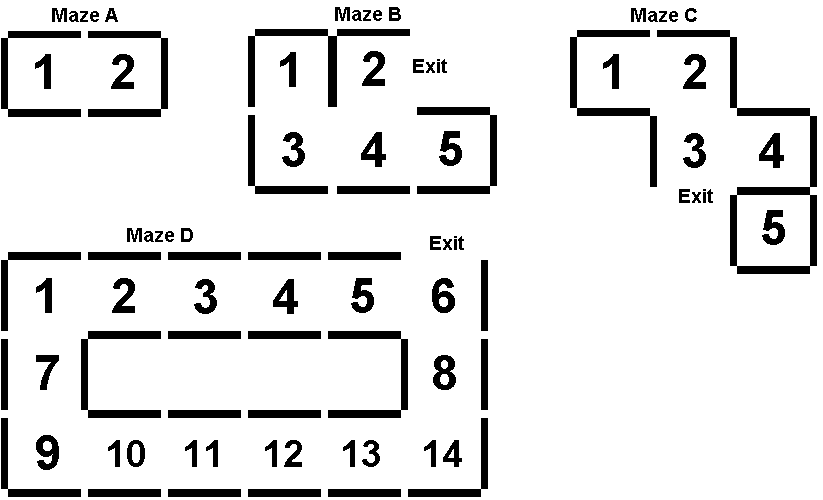
\includegraphics[width=.6\textwidth]{amazing-001.png}
    \caption{(The numbers in the cells above are for illustrative purposes only.)}
\end{center}
\end{figure}

Each side of a cell is labeled with a direction to allow navigation:

\begin{figure}[!h]
\begin{center}
    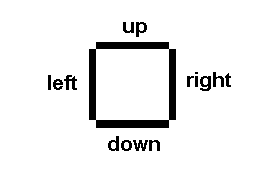
\includegraphics[width=.2\textwidth]{amazing-002.png}
\end{center}
\end{figure}

For each maze, the starting point is someplace in the maze (for example, any of the numbered cells
in the samples above). In the samples above:

\begin{itemize}
\item Maze A has no way out.
\item Maze B has an exit (solution) to the right of cell 2.
\item Maze C has an exit down from cell 3, unless the starting point is cell 5, in which case there is no way out
\item Maze D has an exit up from cell 6.
\end{itemize}

For example, using Maze D above, if the starting point is cell 9, one possible set of directions to get to
the exit would be: \texttt{right}, \texttt{right}, \texttt{right}, \texttt{right}, \texttt{right}, 
\texttt{up}, \texttt{up}, \texttt{up}.

For this problem, you will write a program that finds an exit to a maze. Your program must operate
\emph{interactively}. That is, your program will make a move by providing a direction (right, down, left or up),
and the judging software will send back one of four responses:

\begin{enumerate}
\item \textbf{wall} - indicates that a wall is there and you cannot proceed in that direction
\item \textbf{ok} - indicates that there is door there and you may proceed in that direction to the neighboring cell.
\item \textbf{solved} - indicates that you have successfully found an exit to the maze.
\item \textbf{wrong} - indicates that your program made an error, as discussed below.
\end{enumerate}

If your program determines there is no way out of the maze, you should send the precise string ``\texttt{no way out}'' 
(without the quotes) instead of a direction.
If there is in fact no way out of the maze, you will receive a \textbf{solved} reply.

Your program will receive a \textbf{wrong} indication if any of the following occur:

\begin{enumerate}
\item Your program sends ``\texttt{no way out}'', even though there is a way out.

\item Your program makes the same move (direction) from the same cell twice.
\end{enumerate}

After receiving a \textbf{wrong} or a \textbf{solved} reply, your program should exit.

\section*{Input/Output}

This is an interactive program. The input you receive is a function of the output you generate. All
input and output strings must end in a new-line character. You should never send extra blank lines.

You must make sure that your program's standard output stream is flushed after you output a the new-line 
character that completes a command.
This is accomplished with \texttt{System.out.flush()} in Java, \texttt{stdout.flush()} in Python,
\texttt{fflush(stdout)} in C, and \texttt{cout << flush} in C++.

The first thing your program must do when it starts up is to send its first move 
(\texttt{up}, \texttt{down}, \texttt{right} or \texttt{left}),
followed by a new-line character. It will then wait for a new-line terminated response on the standard
input. The response will be one of \textbf{wall}, \textbf{ok}, \textbf{solved}, or \textbf{wrong}
indication. Your program will then make another move based on the response it received as discussed above. 
This process will repeat until your program receives a \textbf{wrong} or \textbf{solved} indication.

Example (User output in \texttt{Teletype}, Computer judge output in \textbf{Bold}). 
(This sample run has no relationship to the samples shown above).

\begin{center}
\begin{tabular}{|l|}
\hline
\textbf{Sample Run} \\
\hline
\texttt{down} \\
\textbf{wall} \\
\texttt{right} \\
\textbf{wall} \\
\texttt{left} \\
\textbf{wall} \\
\texttt{up} \\
\textbf{ok} \\
\texttt{right} \\
\textbf{ok} \\
\texttt{down} \\
\textbf{ok} \\
\texttt{down} \\
\textbf{wall} \\
\texttt{right} \\
\textbf{wall} \\
\texttt{left} \\
\textbf{wall} \\
\texttt{up} \\
\textbf{ok} \\
\texttt{right} \\
\textbf{solved} \\
\hline
\end{tabular}
\end{center}

It is guaranteed that the maze will not be larger than $100 \times 100$ in any dimension.
